\documentclass[12pt]{article}
%Gummi|065|=)
\usepackage{amsmath, amsfonts, amssymb}
\usepackage[margin=0.5in]{geometry}
\usepackage{xcolor}
%\usepackage{graphicx}
%\usepackage{graphicx}
\newcommand{\off}[1]{}
\DeclareMathSizes{20}{30}{21}{18}

\newcommand{\myhrule}{}

\newcommand{\dash}{
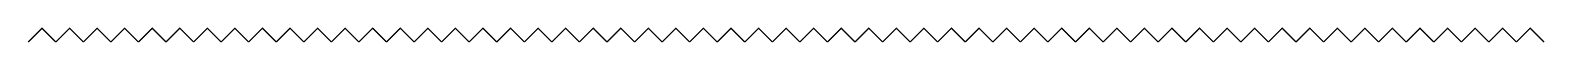
\begin{tikzpicture}[scale=0.35]
\foreach \x in {1,...,55}{
	\draw (\x,-0.25)--(\x+0.5,0.25)--(\x+1,-0.25);
}
\end{tikzpicture}
}

\usepackage{tikz}

\title{\textbf{ Examples: Theta Functions and Poisson Summation}}
\author{John D Mangual}
\date{}
\begin{document}

\fontfamily{qag}\selectfont \fontsize{25}{30}\selectfont

\maketitle

\fontfamily{qag}\selectfont \fontsize{12}{10}\selectfont

\noindent On the one hand, there are many people who know all sorts of things about theta functions.  David Mumford wrote 3 volumes.  They are going to my working examples of modular forms.\footnote{There is also an excellent discussion of Theta Functions and String Theory and Riemann surfaces by the Verlinde brothers, some of which is formalized by Beauville.  There's even a page or two in Feynman's \textbf{Statistical Mechanics}. } \\ \\
\textbf{Ex \#1} Show that if $u(x)$ is a spherical harmonic of degree $\ell$ the generalized theta function
$$ \theta(z; u) = \sum_{m \in \mathbb{Z}^3} u(m) e^{z|m|^2} $$
is a holomorphic cusp form for $\Gamma_0(4)$ of weight $3/2 + \ell$ as long as $\ell \geq 1$.  This will already keep me busy for some time.  The coefficients of this Fourier series are averages over the sphere:
$$  \frac{1}{r_3(n)} \sum_{\xi_1^2 + \xi_2^2 + \xi_3^2 = n} u(\xi) \ll   n^{- 1/28}$$
\textbf{Ex \#2} Show Duke's bound for any exponent $n^\alpha$ with $\alpha < 0$.  Could be $\frac{1}{28}$ or $\frac{1}{100}$\dots Anything.  \\ \\ \\
If I knew what a $\Gamma_0(4)$ holomorphic cusp form was, I might be able to credit Goro Shimura's 1973 paper.  However, he has also written some recent graduate level texts with chaptrs on half-integer weight modular forms.  \\ \\ 
The fraction $\frac{1}{28}$ falls out of difficult calculations involving Kloosterman sums, which I am not going to cite or reproduce.  Therefore, I might expect these bounds to be slightly worse -- if I achieve anything at all.   Instead, I will emphasize elementary\footnote{Duke and Iwaniec also felt there arguments were elementary.  I am sure Duke and Shimura are correct.} computations.\\ \\ 
There are a few easy cases $u(\xi) = 1$ is the spherical harmonic of degree 0 -- it is excluded from discussion.  In fact, $\ell \geq 1$ and $n \gg 1$ should be very large.  Yet:
$$  \frac{1}{r_3(n)} \sum_{\xi_1^2 + \xi_2^2 + \xi_3^2 = n} 1 = 1  $$
and $\xi(x,y,z) = x$ is an odd function.  So that $x^2 + y^2 + z^2 = n$ should have a solution $(x,y,z)$ and $(-x,y,z)$.  Therefore, any odd function such as $u(x,y,z) = x$ should have a vanishing average.  \\ \\
The first non-trivial case -- and we're a far cry from proving Ex \#1 or Ex \#2 -- is $u(x) = x_1^2$ ( notice $u(x) = x_1 x_2$ also vanishes ).  This is not to be understimated that we can switch signs.
$$ (\pm x_1)^2 + (\pm x_2)^2 + (\pm x_3)^2 = n $$
However let's not to forget to try far more basic approaches such as the Hasse Princple.\footnote{Or the mean value theorem! Let $f: \mathbb{R}^3 \to \mathbb{R}$ show that $|\frac{1}{6}\sum_{k \in \{1,2,3\}} f(x \pm dx_k) - f(x)|\ll \partial f (x)$ (this is ambiguous)}

\newpage

\noindent \textbf{Ex \#1A} What is a modular form?  What is a cusp form?  How do we check some crazy series is holomorphic?  I have done many many exercie, and now it's show-time and I've drawn a blank.  There are very good notes of Zagier which gave me my first clue. \\ \\
\textbf{Theta Functions are Modular Forms} His proof is a little bit succinct, and we'll adapt a version from \textit{Methods of Mathematical Physics I} by Courant and Hilbert.  I can almost do it myself.  The Fourier coefficients are merely:
$$ a_m = \int_0^1 \bigg[ \sum_{n = - \infty}^\infty e^{ - n^2 x} \bigg] e^{2\pi i \, m x} \; dx $$
and the we apply the Poisson summation formula $\sum f(n) = \sum \hat{f}(n)$.  We can talk about how to interchange $\sum \int = \int \sum$ and when such an equality can be profitably used.  \\ \\
Now I am going to copy Courtant-Hilbert and here's why.  Consider the theta function over $y + \mathbb{Z}$ with $0 < y < 1$.
$$\phi(y) = \sum e^{- \pi(n + y)^2 \, x}$$
This function is periodic in $y$ -- this has the effect of warpping the complex plane $\mathbb{C}$ about a cylinder $S^1 \times \mathbb{R}$.
$$ \hspace{1.04in}\phi(y) = \sum_{n =0}^\infty e^{- \pi(n + y)^2 \, x}
= \sum_{n =0}^\infty a_n e^{2\pi i n y}$$
The Fourier coeffcients are pretty mechanical to compute for an upper leven Engineer or math student (if they remember integrals)
$$ \hspace{1in} a_m = \int_0^1 \sum_{n = - \infty}^\infty e^{- \pi (n+t)^2 \, x - 2\pi i \, mt} \, dt $$
We are adding a function with many copies of itself shifted by  time $t \mapsto t + n$.  And $\int \sum = \sum \int$:
$$ \hspace{1.04in} a_m = \sum_{n = - \infty}^\infty \int_0^1 e^{- \pi (n+t)^2 \, x - 2\pi i \, mt} \, dt $$
For each term we can move $[0,1]$ to $[n, n+1]$.  Using properties of the Gaussian integral:
$$ a_m = \int_{\infty}^\infty e^{-\pi t^2 x - 2\pi i mt} dt = e^{-\pi n^2 / x}\int_{-\infty}^\infty e^{-\pi x \big(t + i m / x \big)^2} \, dt = \frac{e^{-\pi m^2 / x}}{\sqrt{x}}$$
The Gaussian is (almost) it's own Fouier transform, and therefore, $\theta$ is going to have these modular properties.  How did we know the integral?
$$ 
\int_{-T}^T e^{-\pi x \big(t + i m / x \big)^2} \, dt
+ \int_{T}^{T+im/x} e^{-\pi x \,t ^2} \, dt
- \int_{-T}^{-T+im/x} e^{-\pi x \,t ^2} \, dt
- \int_{-T}^T e^{-\pi x \,t^2} \, dt
= 0 $$
This Gaussian has no poles so this is always zero by Cauchy's theorem.\footnote{Do I believe Cauchy's Theorem here?  If I cut the rectangle $-T, T, T + im/x, -T + im/x $ into very small squares (or triangles) I can verify the integral around these rectangles is zero.  Do I really believe I have the resources to compute all those tiny integrals? Or that the combined errors from all those linear approximations doesn't lead to extra contributions?}.  Then
$$ \theta(x) = \sum_{n = - \infty}^\infty e^{\pi n^2 \, x}= \phi(0) = \frac{1}{\sqrt{x}}
\sum_{n = - \infty}^\infty e^{\pi n^2 / x}
= \frac{1}{\sqrt{x}} \theta(\frac{1}{x})$$

\newpage

\noindent We gave really shifty derivation of Poisson summation in the case of the Gaussian function.  And 3rd year math student should be concerned by any equation of the type:
$$ \sum_{n=0}^\infty \int_0^1 a_n(x) \, dx = 
\int_0^1 \sum_{n=0}^\infty a_n(x) $$
The rearrangement step is a bit worrisome I can try to reproduce it.  This looks somewhat mysterious:
$$\hspace{-0.05in} \sum_{n=-\infty}^\infty \int_0^1 \phi(t + n ) \, dt = \int_{-\infty}^\infty \phi(t) \, e^{-2\pi i\, nt} \, dt $$
This rearrangement trick\footnote{idea} looks almost like the Poisson summation formula itself:
$$ \hspace{0.4in}\sum_{n = - \infty}^\infty \phi(n) = \sum_{n = - \infty}^\infty \int_{-\infty}^\infty \phi(t) e^{- 2\pi i\, t} dt $$
and the Gaussian itself $\phi(t) = e^{-t^2}$ has some extra symmetries as we are learning!  \\ \\
Despite being rather advanced --- a solid review of 3rd and 4th year analysis and geometry yields some partial progress in that direction.


%\fontfamily{qag}\selectfont \fontsize{12}{10}\selectfont


\begin{thebibliography}{}

\item Emil Artin and George Whaples \textbf{Axiomatic characterization of fields by the product formula for valuations} Bull. Amer. Math. Soc.
Volume 51, Number 7 (1945), 469-492.




\end{thebibliography}



\end{document}